\begin{frame}{$K$-théorie contrôlée}
\begin{block}{$C^*$-algèbres filtrée} 
Associer une filtration à une structure géométrique. 
\end{block}
\vspace{0.3 cm}
\begin{itemize}
\item[$\bullet$] Oyono-Oyono \& Yu : utilisation de metriques,
\vspace{0.3 cm}
\item[$\bullet$] Structure coarse : définir la filtration de manière intrinsèque. Le résultat de dépend plus de la métrique, et peut s'appliquer dans des situations purement algébrique (groupes quantiques).
\end{itemize}
\end{frame}

\begin{frame}{$K$-théorie contrôlée}
\[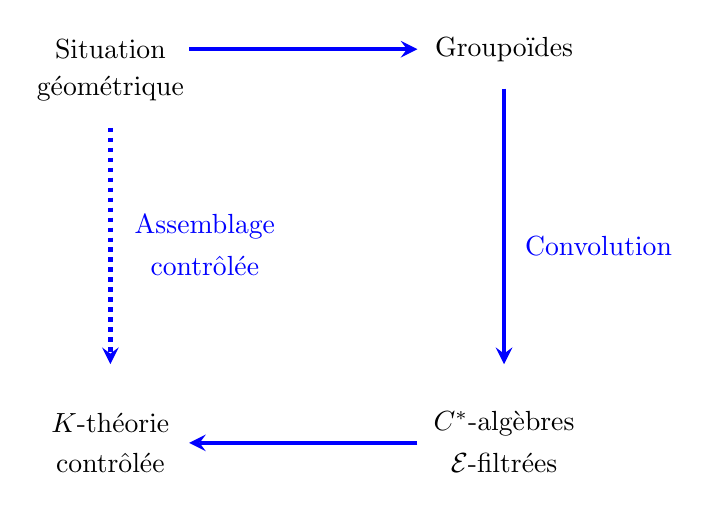
\begin{tikzpicture}
\draw  (0,5) node {Situation};
\draw  (0,4.5) node {géométrique};

\pause

\draw  (5,5) node {Groupoïdes};
\draw [>=stealth, ->,ultra thick, blue] (1,5) -- (3.9,5) ; %->

\pause

\draw  (5,0.25) node {$C^*$-algèbres};
\draw  (5,-0.25) node {$\mathcal E$-filtrées};
\draw [>=stealth, ->,ultra thick,blue] (5,4.5) -- (5,1) ; % |
\draw[blue]  (6.2,2.5) node {Convolution};

\pause 

\draw  (0,0.25) node {$K$-théorie};
\draw  (0,-0.25) node {contrôlée};
\draw [>=stealth, ->,ultra thick, blue] (3.9,0) -- (1,0) ;

\pause
\draw [>=stealth, ->,ultra thick, blue, dotted] (0,4) -- (0,1) ;
\draw[blue] (1.2,2.75) node {Assemblage};
\draw[blue] (1.2,2.25) node {contrôlée};
\end{tikzpicture}\]
\end{frame}

\begin{frame}{$K$-théorie contrôlée}
\begin{definitionfr}
Une structure coarse $\mathcal E$ est un semi-groupe abélien qui est aussi un treillis. \\
\end{definitionfr}
\vspace{0.3 cm}
Rappelons qu'un treillis est un ensemble partiellement ordonné tel que toute paire $(E,E')$ admette un supremum $E\vee E'$ et un infimum $E\wedge E'$.\\
\vspace{0.3 cm}
On note $(E,E')\mapsto E\circ E'$ la loi de composition de $\mathcal E$.
\end{frame}

\begin{frame}{$K$-théorie contrôlée}
\begin{definitionfr}
Une $C^*$-algèbre $A$ est $\mathcal E$-filtrée s'il existe une famille de sous-espaces vectoriels fermés auto-adjoints $\{A_E\}_{E\in\mathcal E}$ de $A$ telle que :
\begin{itemize}
\item[$\bullet$] si $E\leq E'$, alors $A_E\subseteq A_{E'}$,
\item[$\bullet$] pour tout $E,E'\in\mathcal E$, $A_E.A_{E'}\subseteq A_{E\circ E'}$,
\item[$\bullet$] $A$ est l'adhérence de l'union des sous-espaces $A_E$, i.e. $\overline{\cup_{E\in\mathcal E}A_E} = A$.
\item[$\bullet$] si $A$ est unitale, on a de plus $1\in A_E,\forall E\in\mathcal E$.
\end{itemize}
\end{definitionfr}

Si $\mathcal E = \R_+^*$ muni de la somme, on retrouve la définition de Oyono-Oyono et Yu. 
\end{frame}

\begin{frame}{$K$-théorie contrôlée}

Plus de $C^*$-algèbres peuvent être vues commes des $C^*$-algèbres filtrées.

\begin{exple}
Les $C^*$-algèbres de Roe sont filtrées.
\end{exple}

\begin{exple}
Les produits croisés de $C^*$-algèbres par des actions de groupoïdes étales sont filtrées.
\end{exple}

\begin{exple}
Les produits croisés de $C^*$-algèbres par des actions de groupes quantiques discrets sont filtrées.
\end{exple}

\end{frame}

\begin{frame}{$K$-théorie contrôlée}
Soit $\mathcal E$ une structure coarse et $A$ une $C^*$-algèbre $\mathcal E$ filtrée. On définit les $\varepsilon$-$E$-unitaires
\[U^{\varepsilon, E}(A)= \{u\in A_E \text{ t.q. } ||u^*u-1||<\varepsilon\text{ et }||uu^*-1||<\varepsilon \}\]
et les $\varepsilon$-$E$-projections 
\[P^{\varepsilon, E}(A)= \{p\in A_E \text{ t.q. } p=p^*\text{ et }||p^2-p||<\varepsilon \}.\]
\end{frame}

\begin{frame}{$K$-théorie contrôlée}
Comme en $K$-théorie, 
\begin{itemize}
\item[$\bullet$] $P_\infty^{\varepsilon, E}(A)$ est la limite inductive algébrique des $P_n^{\varepsilon, E}(A)$ par rapports aux inclusions
\[\left\{\begin{array}{rcl}
	P^{\varepsilon,E}_n(A) 		& \rightarrow	& P^{\varepsilon,E}_{n+1}(A)\\ 
	p 		& \mapsto 	& \begin{pmatrix}p& 0 \\ 0&0 \end{pmatrix}
\end{array}\right.\]
\item[$\bullet$] $U_\infty^{\varepsilon, E}(A)$ est la limite inductive algébrique des $U_n^{\varepsilon, E}(A)$ par rapports à
\[\left\{\begin{array}{rcl}
	U^{\varepsilon,E}_n(A) 		& \rightarrow	& U^{\varepsilon,E}_{n+1}(A)\\ 
	u 		& \mapsto 	& \begin{pmatrix}u & 0 \\ 0& 1 \end{pmatrix}
\end{array}\right. .\]
\end{itemize}
\end{frame}

\begin{frame}{$K$-théorie contrôlée}
On munit $P_\infty^{\varepsilon, E}(A)\times \N$ et $U_\infty^{\varepsilon, E}(A)$ des relations d'équivalence suivantes:
\begin{itemize}
\item[$\bullet$] $(p,l) \sim (q,l')$ s'il existe une homotopie de quasi-projections $h\in P^{\varepsilon, E}_\infty(A[0,1])$ et un entier $k$ tel que 
\[h(0)=\begin{pmatrix} p & 0 \\ 0 & 1_{k+l'} \end{pmatrix} \text{ and }
h(1)=\begin{pmatrix} q & 0 \\ 0 & 1_{k+l} \end{pmatrix}\]
\item[$\bullet$] $u \sim v$ s'il existe une homotopie de quasi-unitaires $h\in U^{3\varepsilon, E\circ E}_\infty(A[0,1])$ tel que $h(0)= u \text{ and }h(1)=v$.\\
\end{itemize}
\end{frame}

\begin{frame}{$K$-théorie contrôlée}
Si $A$ est unitale,
\begin{itemize}
\item[$\bullet$] $K_0^{\varepsilon,E}(A) = P^{\varepsilon, E}_\infty(A)\times \N / \sim_{\varepsilon,E}$ 
\item[$\bullet$] $K_1^{\varepsilon,E}(A) = U^{\varepsilon, E}_\infty(A) / \sim_{\varepsilon,E}$.
\end{itemize}

Si $A$ n'est pas unitale,  
\[K_0^{\varepsilon,E}(A) = \{[p,l]_{\varepsilon,E} : p\in P^{\varepsilon,E}_\infty (\tilde A), l\in \N \text{ s.t. rank}(\kappa_0(\rho_A(p)))=l \}\]
et $K_1^{\varepsilon,E}(A)$ est défini par $U_\infty^{\varepsilon,E}(\tilde A)/ \sim_{\varepsilon,E}$.\\

\begin{definitionfr}
La $K$-théorie contrôlée d'une $C^*$-algèbre filtrée $(A,\mathcal E)$ est la famille de groupes abéliens 
\[\hat K_0(A) = (K_0^{\varepsilon,E}(A))_{\varepsilon\in (0,\frac{1}{4}),E\in\mathcal E} \text{ et } \hat K_1(A) = (K_1^{\varepsilon,E}(A))_{\varepsilon\in (0,\frac{1}{4}),E\in\mathcal E}.\]
\end{definitionfr}
\end{frame}

\begin{frame}{$K$-théorie contrôlée}
$\bullet$ Pour tout $\varepsilon <\varepsilon'$ et $E\subseteq E'$, on dispose de morphismes 
\[\iota_{\varepsilon,E}^{\varepsilon',E'} : K^{\varepsilon,E}(A)\rightarrow K^{\varepsilon',E'}(A) \]
tels que $\iota_{\varepsilon',E'}^{\varepsilon'',E''}\circ \iota_{\varepsilon,E}^{\varepsilon',E'} = \iota_{\varepsilon,E}^{\varepsilon'',E''}$ et $\iota_{\varepsilon,E}^{\varepsilon,E}= id_{K^{\varepsilon,E}(A)}$.\\
\vspace{0.3 cm}
$\bullet$ Pour tout $\varepsilon $ et $E\in\mathcal E$, on dispose de morphismes 
\[\iota_{\varepsilon,E} : K^{\varepsilon,E}(A)\rightarrow K(A) \]
tels que $\iota_{\varepsilon',E'}\circ \iota_{\varepsilon,E}^{\varepsilon',E'} = \iota_{\varepsilon,E}$.\\
\vspace{0.3 cm}
$\bullet$ Pour tout élément $x\in K(A)$ et tout $\varepsilon\in (0,\frac{1}{4})$, il existe $E\in\mathcal E$ et $y\in K^{\varepsilon,E}(A)$ tel que $x=\iota_{\varepsilon,E}(y)$.
\end{frame}

\begin{frame}{$K$-théorie contrôlée}
$\bullet$ Une paire de contrôle $(\alpha,\rho)$ est donnée par $\alpha\in (0,\frac{1}{4})$ et $k : (0,\frac{1}{4\alpha})\rightarrow \N $ croissante.
\begin{definitionfr}[Morphisme contrôlé]
Un morphisme $(\alpha,k)$-contrôlé $\hat F : \hat K(A) \rightarrow \hat K(B)$ est une famille de morphismes 
\[F^{\varepsilon,E}: K^{\varepsilon,E}(A) \rightarrow K^{\alpha\varepsilon,k_\varepsilon. E}(B)\] 
compatible avec les $\iota_{\varepsilon,E}^{\varepsilon',E'}$.
\end{definitionfr}
\vspace{0.3 cm}
On dit que $\hat F$ induit $F : K(A)\rightarrow K(B)$ en $K$-théorie si 
\[\iota_{\alpha \varepsilon,k_\varepsilon E}\circ F^{\varepsilon,E}=F.\]
\textbf{Remarque :} Notion d'isomorphisme contrôlé et de suite exacte contrôlée.
\end{frame}

\begin{frame}{$K$-théorie contrôlée}
$\bullet$ Tout $*$-homomorphisme filtré $\phi; A\rightarrow B$, i.e. $\phi(A_E)\subseteq B_E$, induit un morphisme contrôlé 
\[\phi_* : \hat K(A)\rightarrow \hat K(B).\]
$\bullet$ Morita équivalence : $A \rightarrow A\otimes\mathfrak K ; a\mapsto a\otimes e$ induit un isomorphisme
\[K^{\varepsilon,E}(A)\rightarrow K^{\varepsilon,E}(A\otimes\mathfrak K).\]
$\bullet$ Pour toute suite exacte complètement filtrée, il existe une suite exacte contrôlée à $6$ termes, ainsi qu'un bord contrôlé.\\
\vspace{0.3 cm}
$\bullet$ Périodicité de Bott contrôlée : $p\mapsto 1+(e^{2i\pi }-1)p$ induit un isomorphisme contrôlé
\[\beta_A :\hat K_0(A) \rightarrow  \hat K_1(SA).\]

%il existe une paire de contrôle $(\alpha_\beta,k_\beta)$ et un morphisme $(\alpha_\beta,k_\beta)$-contrôlé
%\[\beta_A : K^{\varepsilon, E}(SA)\rightarrow K^{\alpha_\beta\varepsilon, k_\beta(\varepsilon) . E}(A)\]
%qui admet un inverse contrôlé $D_A$.
\end{frame}












































